% -*- coding: utf-8 -*-


\newcounter{questioncount}
\setcounter{questioncount}{0}
\newcommand{\question}{\addtocounter{questioncount}{1}\paragraph{Question \Alph{questioncount}.}}
\newcommand{\commentaire}[1]{}
\newcommand{\pt}[1]{\fbox{$#1 \operatorname{pt}$}}
%%%% Bareme

\setlength{\marginparpush}{2pt}
\newcounter{totalpointsint}
\newcounter{tempsint}
\setcounter{totalpointsint}{0}
\newcounter{minutesparpoint}
\newcounter{degresint}
\newcounter{anglefancyclock}
\newcounter{dureeexamheures}
\newcommand{\BaremeSurTroisH}{
\setcounter{minutesparpoint}{9}
\setcounter{dureeexamheures}{3}
}
\newcommand{\BaremeSurDeuxH}{
\setcounter{minutesparpoint}{6}
\setcounter{dureeexamheures}{2}
}
\newcommand{\DebutBareme}{
\setcounter{anglefancyclock}{90}
}
\setcounter{minutesparpoint}{1}
%\BaremeSurTroisH
\DebutBareme
\newcommand{\fancyclockmin}[1]{
\setcounter{tempsint}{\theminutesparpoint*\real{#1}}
\setcounter{degresint}{\thetempsint*6}
\setcounter{anglefancyclock}{\theanglefancyclock-\thedegresint}
\noindent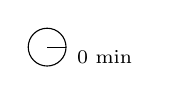
\begin{tikzpicture}[scale=.8]
    \draw (0,0) circle (3mm);
\ifnum\theanglefancyclock<0          % modulo de l'angle
\addtocounter{anglefancyclock}{360}  %
\fi                                  %
%\draw (0mm,0mm) node [black!30] {\bf\Large\thedureeexamheures};
%\draw (0mm,0mm) node [black!25] {\Large\thedureeexamheures};
\filldraw[rotate=\theanglefancyclock] (0,0) -- (0:3mm) arc (0:\thedegresint:3mm) -- cycle;
%\draw (3.2mm, 1.5mm) node[anchor=west] {\scriptsize #1~pt};
\draw (3.2mm, -1.5mm) node[anchor=west] {\scriptsize \thetempsint~min};
  \end{tikzpicture}
% \tiny
% \begin{tabular}{@{}r@{} @{}l@{}}
%  #1&~pt\\
%  \thetempsint&~min
% \end{tabular}
}

\newcommand{\bareme}[1]{%
\addtocounter{totalpointsint}{10*\real{#1}}\marginpar{%
\footnotesize\fancyclockmin{#1}
%\hfill\thetotalpointsint
}}
\newcommand{\Bareme}[1]{\marginpar{\fbox{\small tot: #1 pt}\hfill}}


\entete{Algorithmique et programmation (I3) contrôle}
\vspace{-0.5cm}

\noindent\textbf{Durée :} 1 heure 20 minutes. Aucun document autorisé.

\section{Étude et modification de programme \emph{(5 points)}} 

Le programme suivant comporte deux erreurs :\bareme{15}
\begin{listing}{1}
#include <stdlib.h>
#include <stdio.h>

int factorielle(int n);

int main () {
  /* test de factorielle */
  printf("Test (doit donner 120) : %d\n", factorielle(5));

  return EXIT_SUCCESS;
}

double factorielle(int n) {
  int res;
  int i;

  i = 1;
  while (i <= n) {
    res = res * i;
    i = i + 1;
  }

  return res;
}
\end{listing}
\question L'une des erreurs empêche la compilation du programme. Corriger.  

\question L'autre erreur
génère un calcul faux. Corriger.
\question Lignes 17 à 21, il aurait été plus naturel d'employer
une autre structure de contrôle que le \C{while}. Quelle structure, et
qu'écririez-vous à la place de ces lignes ?


\section{Sans fonctions \emph{(5 points)}}

\question Soit un tableau \C{t} d'entiers, que vous initialiserez à
des valeurs de votre choix, d'une taille donnée par un constante \bareme{15}
symbolique \C{N}. Écrire un programme qui demande un entier \C{seuil}
à l'utilisateur puis affiche les éléments de \C{t} supérieurs ou égaux
à ce seuil. Par exemple, si les éléments de \C{t} sont les entiers $4,
6, -1, 6, 7, 4$ et si l'utilisateur fixe le \C{seuil} à $6$ alors le
programme affichera $6, 6, 7$.

\section{Canard aux olives \emph{(10 points)}}
Vous disposez d'un recueil de recettes avec, pour chaque recette, un
temps de préparation et un temps de cuisson. Pour les viandes le temps
de cuisson est donné par kilogramme. Vous souhaitez produire une application
qui calculera la durée réelle de cuisson et la durée totale de \bareme{50}
réalisation de la recette (préparation et cuisson). Aujourd'hui, il
vous faut mettre au point la partie affichage et calcul des durées, en
travaillant sur un exemple de recette.

\question Déclarer un type \verb+duree_t+ permettant de stocker des
durées exprimées en heures, minutes, secondes (valeurs entières) et
définir une procédure \C{afficher} permettant d'afficher une durée, comme dans l'exemple.

\question Déclarer et définir une fonction \C{normaliser} mettant une durée sous la forme usuelle où le nombre de secondes et le nombre de minutes sont inférieurs à 60. Par exemple, la durée \C{1h 75min 64sec} sera normalisée en \C{2h 16min 4sec}.

\question Déclarer et définir une fonction \C{add}  permettant d'additionner des durées et une fonction \C{mult} permettant de multiplier une durée par un  facteur fourni en paramètre (un double). Ces fonctions rendront des résultats normalisés.

\question Compléter la partie calcul du programme.
{\begin{small}
\begin{verbatim}
int main() {
  duree_t prep = {0,30,0};   /* tps de preparation  30 minutes */
  duree_t par_kg = {0,52,0}; /* tps de cuisson par kilo 52 minutes */
  double poids = 1.94;       /* poids du canard 1.94 kg */

  duree_t cuisson;           /* temps reel de cuisson, à calculer */
  duree_t realisation;       /* temps total de realisation, à calculer */
  
  printf("**Recette du canard aux olives.**");
  printf("\nTemps de préparation : ");    
  afficher(prep);
  printf("\n\n* Temps de cuisson ");
  printf("\nPar kg : ");
  afficher(par_kg);

  /* ici il faut ajouter le calcul des durees reelles */

  printf("\nPour un canard de %lg kg : ", poids);
  afficher(cuisson);
  printf("\nTemps total de la recette : ");
  afficher(realisation);

  return EXIT_SUCCESS;
}
\end{verbatim}

\tikzstyle{information text}=[rounded corners,fill=black!10,inner sep=1ex]

~\hfill
\begin{tikzpicture}
\path[use as bounding box] (0,0) rectangle (0, 0);
\draw[xshift=-8cm, yshift=0cm] node [right,text width=8cm,style=information text] {
Exemple d'affichage.
\begin{verbatim}
**Recette du canard aux olives.**
Temps de préparation :  0h 30min  0sec
 
* Temps de cuisson 
Par kg :  0h 52min  0sec
Pour un canard de 1.94 kg :  1h 40min 52sec
Temps total de la recette :  2h 10min 52sec
\end{verbatim}
};
\end{tikzpicture}
\end{small}}
%\newpage
%\hfill Total des points (bonus inclus) : \thetotalpointsint


%%% Local Variables: 
%%% mode: latex
%%% TeX-master: "final"
%%% End: 